
%(BEGIN_QUESTION)
% Copyright 2010, Tony R. Kuphaldt, released under the Creative Commons Attribution License (v 1.0)
% This means you may do almost anything with this work of mine, so long as you give me proper credit

A process called {\it delayed coking} is used in the oil refining industry to convert heavy oils and tars into higher-valued petroleum products.  A process vessel called a {\it coke drum} has a removable lid held down by a series of bolts, and alternatively by a hydraulic ram.  When it comes time to open up the coke drum, the hydraulic ram is pressurized to maintain adequate force on the coke drum lid, the bolts are removed, and then the ram's fluid pressure is reduced until the lid springs open from the force of the gas pressure inside the coke drum:

$$\includegraphics[width=15.5cm]{i04683x01.eps}$$

Calculate the hydraulic pressure necessary to hold down the lid on the coke drum when the gas pressure inside the drum is 5 PSI and all hold-down bolts have been removed from the lid.  Assume a lid diameter of 30 inches, and a ram piston diameter of 4 inches.  Hint: sketch a right triangle, representing forces as side lengths on the triangle -- the ram's diagonal force will translate into both a horizontal force on the lid (which you may ignore) and a vertical force on the lid (which is what we're interested in here).

\vskip 10pt

Hydraulic $P$ = \underbar{\hskip 50pt} PSI

\vskip 20pt \vbox{\hrule \hbox{\strut \vrule{} {\bf Suggestions for Socratic discussion} \vrule} \hrule}

\begin{itemize}
\item{} Which direction will the horizontal force component be exerted on the lid?
\item{} Identify the potential hazards of a hydraulic oil leak in this system.  Compare the effects of a slow leak (e.g. a leaky fitting connecting the hose to the ram) versus a catastrophic leak (e.g. the hose bursting from excess pressure).
\end{itemize}

\underbar{file i04683}
%(END_QUESTION)





%(BEGIN_ANSWER)

With a piston diameter of 4 inches, a hydraulic pressure of 456.83 PSI is necessary to generate 5740.6 pounds.  This is a {\it minimum} pressure, for safety reasons.  More than 456.83 PSI won't do any harm, but less than this amount will fail to hold down the lid!

%(END_ANSWER)





%(BEGIN_NOTES)

The force on the lid from the coke drum's internal pressure of 5 PSI will be 3534.3 pounds, which is how great the ram's {\it vertical} force component must be to successfully hold down the lid when all the bolts have been removed.  The ram's angle of 38 degrees from horizontal means the vertical force component will only be 0.6157 of its diagonal force (sine of 38$^{o}$ = 0.6157).  This necessitates a direct ram force of 5740.6 pounds.

$$\includegraphics[width=15.5cm]{i04683x02.eps}$$

With a piston diameter of 4 inches (area = 12.566 square inches), the necessary hydraulic pressure for the ram to exert 5740.6 pounds of force will be:

$$P = {F \over A} = {5740.6 \hbox{ lb} \over 12.566 \hbox{ in}^2} = 456.83 {\hbox{lb} \over \hbox{in}^2} = 456.83 \hbox{ PSI}$$

%INDEX% Physics, fluids: pressure, force, and area
%INDEX% Process: delayed coker drum lid hydraulic hold-down

%(END_NOTES)

